\appendix
\section{Convolutional Parametrizations}

In the main paper, we experimented with fully connected architectures
for representing manifold parametrizations.
However, parametrizations represented by convolutional architectures
also induce a prior useful for manifold reconstruction tasks.
In this section, we show experiments with denoising and single-view
reconstruction.
We start by defining a \texttt{ConvBlock}, which consists of a bilinear upsampling layer followed by a 2D-conv, batch normalization~\cite{batchnorm} and Leaky ReLU activation (slope=$0.2$).
Every convolutional layer uses filter size $3 \times 3$, stride $1$ and the number of filters is exactly half the number of its input channels.
In other words, at every \texttt{ConvBlock}, the output tensor spatially doubles the size of its input tensor, but only has half the number of channels.
This pattern follows throughout the whole network, except for the last layer, where the output layer always have 3 channels, representing the $(x,y,z)$ point coordinates.

\subsection{Denoising}

The denoising experiments follow the same procedure described in the
main paper, except for the network architecture.
Instead of using a fully connected model, we employ a network with 3 \texttt{ConvBlock}s,
starting from an input tensor with shape $4\times4\times512$ whose values are drawn from
a standard gaussian distribution.
The output of each parametrization is a tensor with shape $32\times32\times3$, which we can treat
as a point cloud with 1024 and use Chamfer distance in the same way as described in Section 5.
We also use the position of the points in the output tensor to define the local neighborhood
utilized in the stretch regularization.
Results are presented in Figure~\ref{fig:rebuttal}.
As we can see, convolutional parametrizations also induce a useful prior for manifold
reconstructions and, similarly to the other parametrizations, it is significantly
better than the baselines.
Quantitatively, using convolutional parametrizations in the denoising yields slightly
worse results than using fully connected networks -- in terms of Chamfer distance, 4.58$\times10^{-4}$ vs. 4.48$\times10^{-4}$.


\begin{figure}[ht!]
    \centering
    \vspace{-10pt}
    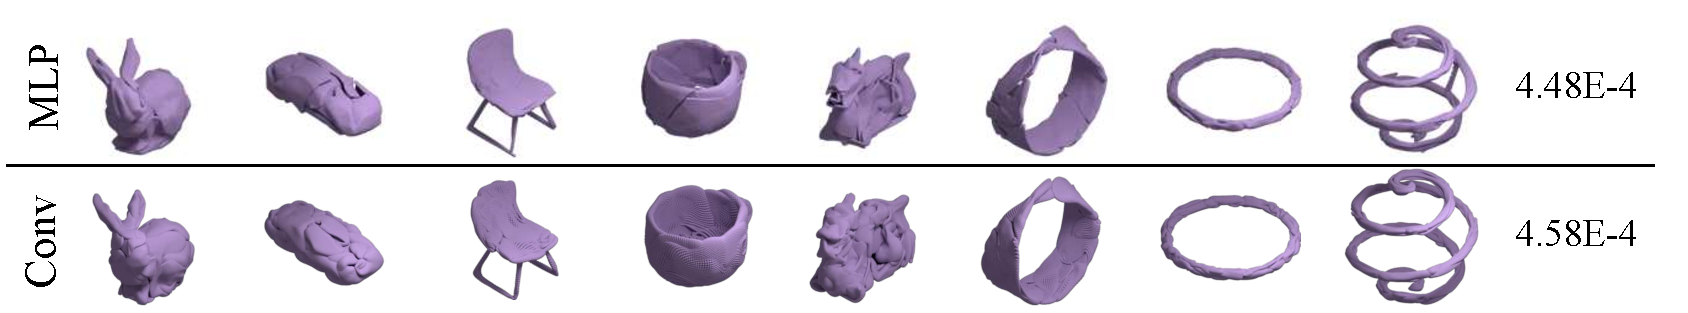
\includegraphics[width=1.0\linewidth]{imgs/conv_denoising.pdf}
    \vspace{-20pt}
    \caption{\label{fig:rebuttal}\small
    Comparison of Conv and MLP networks for denoising.
    Average error across shapes to the right. Both models use 8
    parametrizations and stretch regularization. Zoom for details.
    }
\end{figure}


\subsection{Single-view Reconstruction}

\begin{figure*}[t]
\centering
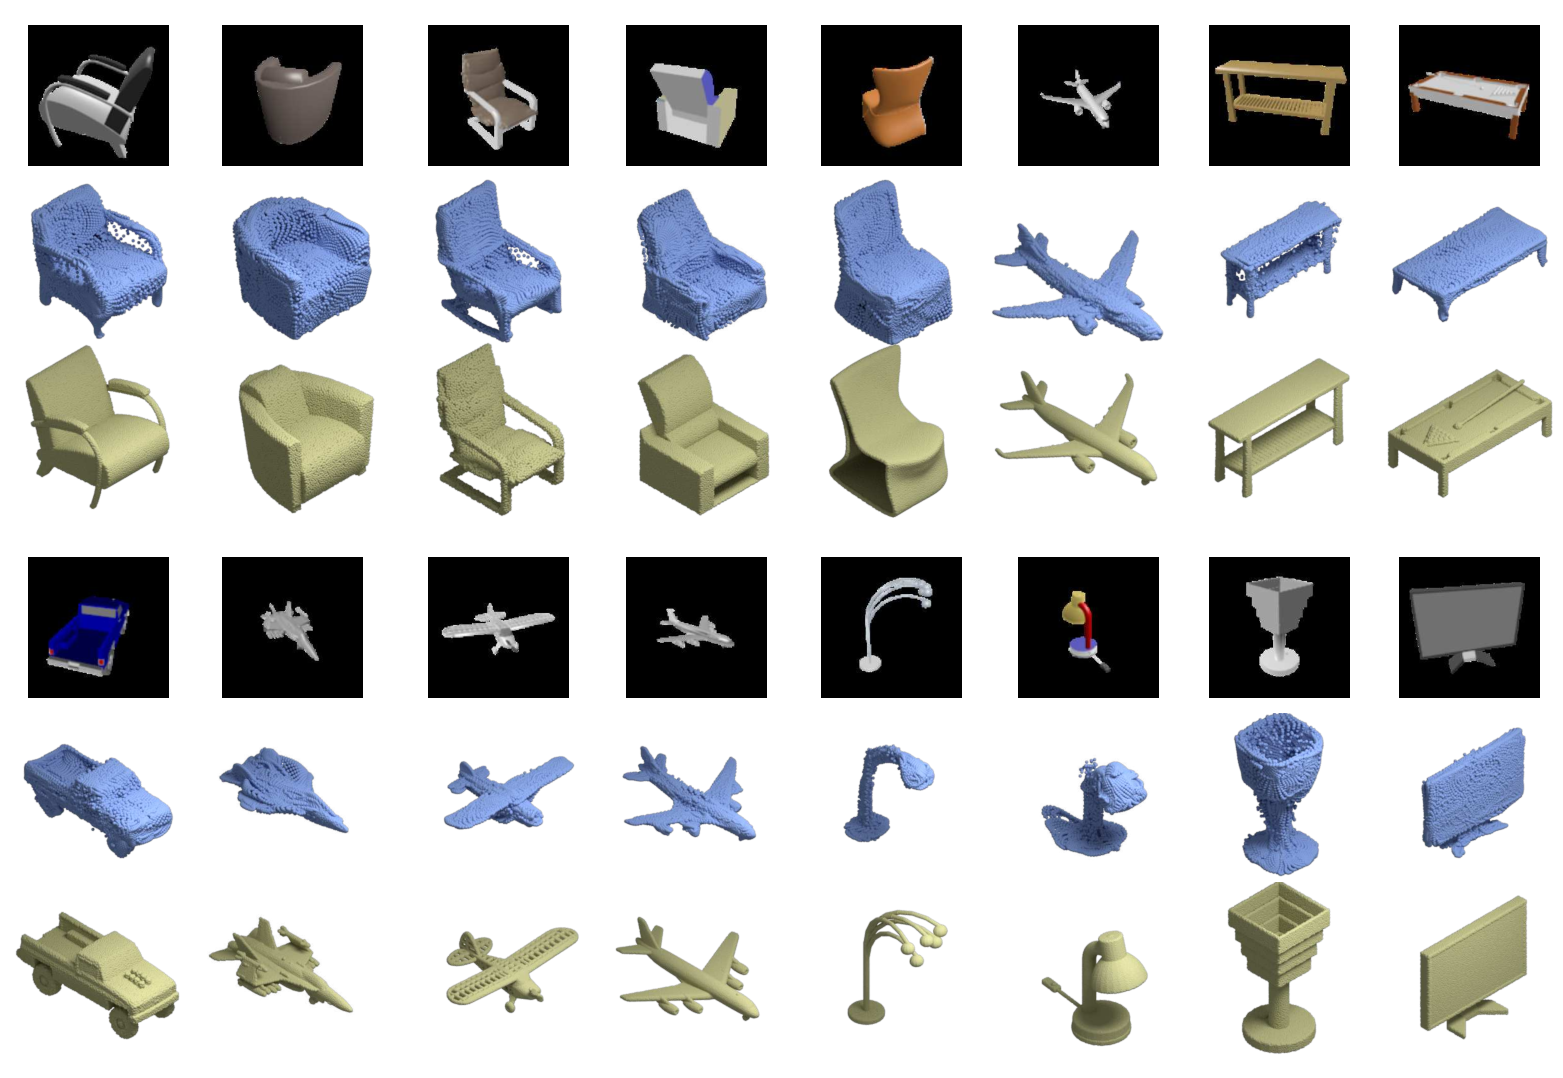
\includegraphics[width=0.9\linewidth]{imgs/data.pdf}
\vspace{-8pt}
	\caption{\label{fig:data} \small
	\textbf{Image-to-shape reconstruction results from the test set.} The images shown are the input (black background), our results (32K points, rendered blue), and ground truth (rendered in light green). Qualitatively, our method is able to generate high-resolution point clouds faithfully capturing fine geometric details such as the chair legs, arms, airplane engines, monitor stands etc.}
	
\end{figure*}

In this subsection we present quantitative and qualitative results for single-view image-to-shape using convolutional paramterizations.
We also train a convolutional decoder with stretch regularization on the single-view reconstruction benchmark~\cite{choy20163d}.
This follows the same experimental setup as previous papers \cite{fan2016point, choy20163d, atlasnet, mrt18}.
However, unlike AtlasNet~\cite{atlasnet}, our network is trained in one stage, without the need to
train the decoder in an auto-encoder setting before fine-tuning it with an image CNN in a second step.
We used Adam optimizer~\cite{kingma2014adam} with learning rate of $10^{-3}$. 
The model is trained for 40 epochs and the learning rate is divided by 2 every 5 epochs.
We use ResNet-18 as image encoder and 32 convolutional parameterizations.
Even though we use more parameterizations than AtlasNet, the total number of parameters is smaller (see Table~\ref{tab:param}.
The evaluation results per category are presented in Table~\ref{tab:svr}.
Compared to MRTNet, our model performs better in 12 out of 13 categories. Compared to AtlasNet, our method is better or ties (the firearm category) in 7 out of 13 categories.
Overall our approach outperforms AtlasNet in per-category mean by 0.21, a relative improvement of 4.4\%. Also note that our model outperforms AtlasNet mainly in categories with
a large number of examples (tables, cars, airplanes, chairs). As a result, if average over instances, our method has a per-instance mean of 4.0, vs. 4.38 by AtlasNet -- a relatively improvement of  8.7\%.

\begin{table*}[h!]
\centering
{
\small
  \begin{tabular}{l|c|c|c|c|c|c|c|c|c|c|c|c|c||c}
   &  pla. &  ben. &  cab. &  car &  cha. &  mon. &  lam. &  spe. &  fir. &  cou. &  tab. &  cel. &  wat. &  \textbf{mean} \\
  \hline
 AtlasNet~\cite{atlasnet} &
2.17 &
\textbf{3.39} &
\textbf{3.93} &
3.40 &
4.56 &
\textbf{5.05} &
12.24 &
8.79 &
\textbf{2.15} &
\textbf{4.58} &
4.15 &
\textbf{3.25} &
3.93 &
4.74\\
 
 MRTNet~\cite{mrt18} &
2.25 &
3.68 &
4.73 &
\textbf{2.55} &
4.06 &
6.07 &
11.15 &
8.84 &
2.25 &
4.98 &
4.45 &
3.72 &
3.64 &
4.80\\



Ours (32 dec.)&
\textbf{2.06} &
3.40 &
4.46 &
2.60 &
\textbf{3.76} &
5.94 &
\textbf{10.66} &
\textbf{8.38} &
\textbf{2.15} &
4.64 &
\textbf{3.96} &
3.45 &
\textbf{3.40} &
\textbf{4.53} \\
  \end{tabular}
  }
\caption{\small \textbf{Quantitative results for single-view image-to-shape reconstruction.} The table reports Chamfer distance metric (scaled by $10^3$) computed per category, and the mean of all categories.
For each method 4K points were used to compute the distance. %
  }
  \label{tab:svr}
\end{table*}

\paragraph{Ablation studies.} Table~\ref{tab:alt} shows a quantitative comparison between a few architectural variations.
We start by analyzing a variation of our network that generates the same number of points (using a single decoder) as MRTNet (4K points) and the same image encoder (vgg-16).
The performance of this variation is 0.05 worse than MRTNet, but it has an order of magnitude less parameters than MRTNet.
Another variation is to still use a single decoder but generate a higher-resolution point cloud (16K points).
This variation results in improved Chamfer distance, by 0.1, than the first variation, indicating that the increased resolution does improve reconstruction accuracy. Again, even when the number of generated points is higher than 4K, our evaluation is done by randomly selecting 4K points, for fair comparison. The last row in the table is our default setting (32 decoders outputting a total of 32K points). 
The number of network parameters are reported in Table~\ref{tab:param}. Even though the number of points our network generates is 8 times that of MRTNet, its size is only about 1/6 of MRTNet, since our network does not need to represent multiple resolutions at each layer. Compared to AtlasNet, our network is about 1/3 of its size, due to the efficiency of using a fully convolutional architecture. Despite using a much smaller number of parameters, our network outperforms MRTNet (in terms of Chamfer distance metric) by 0.27, and AtlasNet by 0.21.


\begin{table}
\centering
{
\begin{tabular}{|l|c|c|}
    \hline
    Architecture &  mean/cat. & mean/inst. \\
    \hline
    MRTNet & 4.80 & 4.26 \\
    1 dec./vgg16/4k & 4.85 & 4.30\\
    1 dec./res18/16k & 4.75 & 4.22\\
    32 dec./res18/32k & \textbf{4.53} & \textbf{4.00}\\
    \hline
\end{tabular}
}
\caption{\label{tab:alt} \small
    \textbf{Architecture variations and evaluation results.} The table reports per-category mean and per-instance mean for MRTNet, and three variations of our methods: single decoder with 4K output points, 16K output points, and 32 decoders with 32 output points. For all cases, the Chamfer distance is calculated using 4K sample points, and results are scaled by $10^3$.
}
\end{table}

\begin{table}
\centering
{
\begin{tabular}{|l|c|}
    \hline
    Method &  \#parameters \\
    \hline
    AtlasNet & 42.6M \\
    MRTNet & 81.6M \\
    \hline 
    Ours (1 dec.) & 2.49M \\
    Ours (1 residual dec.) & 5.79M \\
    Ours (32 dec.) & 14.5M  \\
    \hline
\end{tabular}
}
\caption{\label{tab:param} \small
    \textbf{Comparing the \# of network parameters.}
}
\end{table}

\paragraph{Qualitative Results.} Figure~\ref{fig:data} shows image-to-shape reconstruction results for images from the test dataset. Overall our method is able to accurately capture fine geometric details such as the chair legs, arms, airplane engines, monitor stands etc. The number of points (32K) is considerably higher than previous work (e.g. 1K by~\cite{fan2016point} and 4K by~\cite{mrt18}). Some specific shapes, such as lamps and jet fighters, present significant challenges for the network as the input images do not contain all the visual details. Nonetheless our method is able to produce a reasonable approximation.


\paragraph{Test on real images.} The test set images are synthetically rendered and as such they look similar to the training images. To evaluate our method on real images we use photos downloaded from the Internet, as shown in~\cite{mrt18}. They are processed by removing the background so only the foreground object remains. Figure~\ref{fig:toy} shows the results. The top row in the figure shows furniture objects, which demonstrate that even though the network is trained using synthetic images rendered with artificial lighting and materials, the model is able to generalize well to real shading, lighting, and materials. The second row shows additional objects where the shading is considerably different from training images. In particular, the last image (desktop computer) is in a category that the training has never seen. Nonetheless the reconstructed shape is reasonable.



\begin{figure*}[t]
\centering
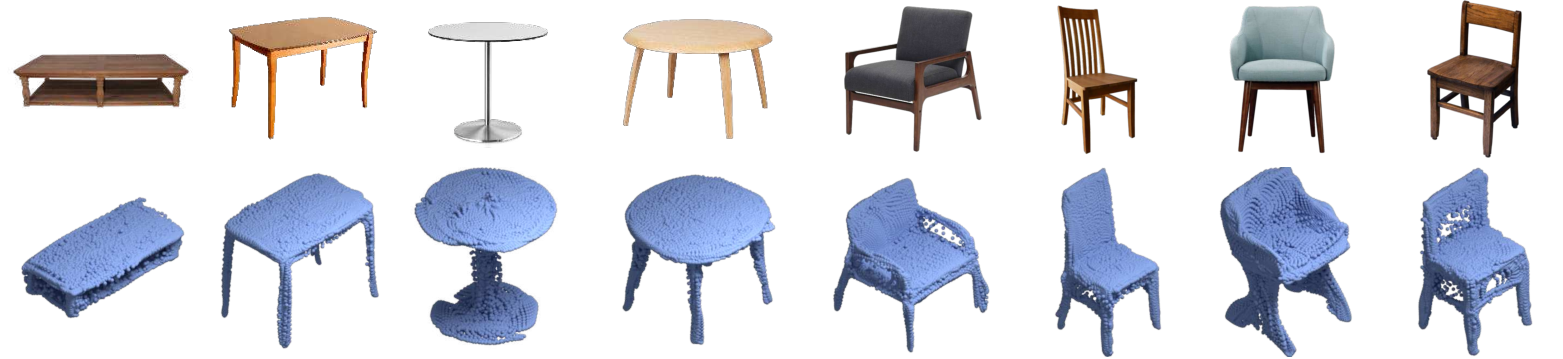
\includegraphics[width=0.9\linewidth]{imgs/furniture.pdf}
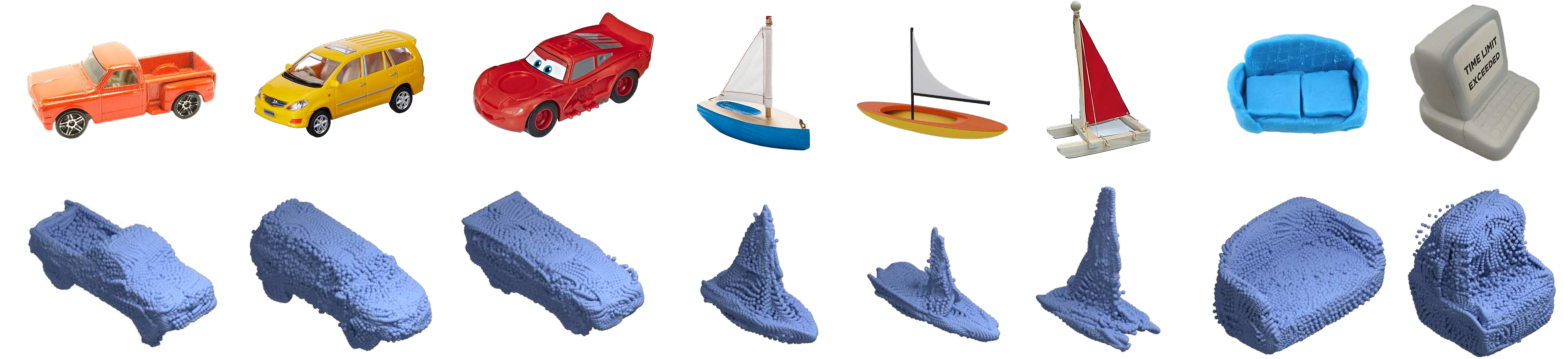
\includegraphics[width=0.9\linewidth]{imgs/toys.pdf}
	\caption{\label{fig:toy} \small
	\textbf{Image-to-shape reconstruction results on Internet photos.} We test our method on real photos downloaded from the Internet and the results are rendered in blue. 
    The test images here are considerably different from the training set. Our method achieves reasonable results with accurate geometric details. The last image (computer) represents a category that has not been seen during training.
    }
\end{figure*}

\begin{figure*}[h!]
\centering
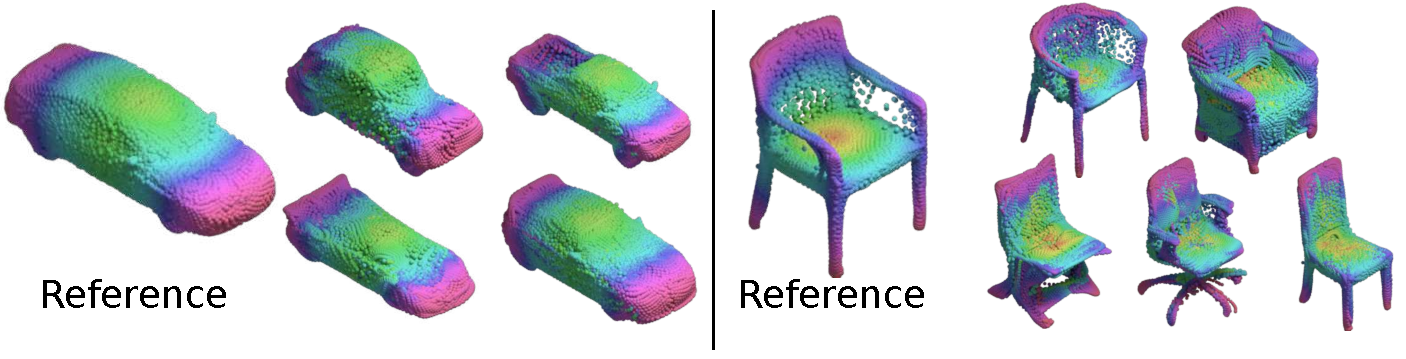
\includegraphics[width=0.8\linewidth]{imgs/corresp.pdf}
	\caption{\label{fig:corresp} \small
	\textbf{Visualizing Shape Correspondences.}
	Our network learns approximate shape correspondences even though the training is not supervised with such information. The shapes shown here are generated by 32 decoders.
	}
\end{figure*}

\paragraph{Shape correspondence.} Once trained, our network learns to generate shapes with corresponding structures.
We demonstrate this with the following experiment.
First, we randomly select a point cloud generated by our network and call it a reference shape.
Then, we assign every point in the reference shape a color, where the hue is computed based on the point's distance to the center of gravity of the object.
Then this color assignment is propagated to the other point clouds, such that a point at index $(i,j)$ in the output tensor is assigned the same color as the point on the reference shape at the same index.
The resulting colorized point clouds are shown in Figure~\ref{fig:corresp}. Similar color indicates similar index range in the output tensor.
Note that even though the network is not trained explicitly with point correspondences as
supervisory signal, it learns to generate corresponding parts in the same
regions of the output tensor, as can be seen around
the tips of the chairs' arms,  legs and  seats.


\section{Limiting distribution for the curvature}

We start by parameterizing the derivative of a space curve $\dot{x} = \cos(f(t))$ 
and $\dot{y} = \sin(f(t))$ where $f$ is a neural network. 
From the standard analysis we know that $f(t)$ converges to a Gaussian with mean $\mu$ and kernel $k(\cdot,\cdot)$. 
Without loss of generality we can assume that the mean $\mu$ is such that $\cos(\mu) \neq 0$ and $\sin(\mu)\neq 0$. 
This can be achieved by adding a fixed bias term $\mu$ to the output of the last layer. 
To compute the limiting distribution of $\ddot{x}$ and $\dot{y}$ we apply the first order delta method to obtain:

\begin{align}
\dot{x} &\rightarrow {\cal N} (\cos(\mu), \sigma^2\sin^2(\mu)), \\
\dot{y} &\rightarrow {\cal N} (\sin(\mu), \sigma^2\cos^2(\mu)). 
\end{align}

Note we can only apply the first order delta method when the derivatives are not zero. 
Hence we assumed that $\mu$ is set to be a quantity which has this property. 
Otherwise we need the second-order delta method and the resulting distribution would be $\chi^2$ for one of the derivatives.

Since the derivative is a linear operator it follows that $\ddot{x}$ and $\ddot{y}$ are also GPs. 
The curvature formula for a arc-length parameterized space curve is $\kappa ^2= \ddot{x}^2 + \ddot{y}^2$. 
From this it follows that $\kappa^2$ is a $\chi^2$ random variable.




\paragraph{Graph parameterization.}

We also analyze the case where the curve is the graph of a one-dimensional function, i.e., $x=x$,$y=f(x)$. 
In this case the curvature can be written as $\kappa=\ddot{f}/((1+\dot{f}^2)^\frac{3}{2})$. 
Once again all the derivatives $\dot{f}$ and $\ddot{f}$ are Gaussian random variables. 
Assume that $(\dot{f}, \ddot{f})$ are distributed according to $N(0,\Sigma)$. Here $\Sigma = [\sigma_{\dot{f},\dot{f}}, \sigma_{\dot{f}\ddot{f}}; \sigma_{\dot{f}\ddot{f}}, \sigma_{\ddot{f}\ddot{f}} ]$ denoting the joint covariance distribution.
Applying the delta method with $g(a, b) = b/(1+a^2)^{3/2}$, we get that $k$ is distributed as a Gaussian random variable $N(0, \nabla g^T \Sigma \nabla g)$. Since $\nabla g(a, b) |_{0,0} = [0, 1]$, we have $k \rightarrow N(0, \sigma_{\ddot{f}\ddot{f}})$.


{\small
\bibliographystyle{ieee_fullname}
\bibliography{egbib,mrnet}
}
\end{document}
